\section{Dokumentacja techniczna}
\subsection{Hardware}
\subsubsection{Ogólne parametry robota:}
Wymiary zewnętrzne: 180mm x  134mm x 84mm

Masa: 0,5 Kg

\subsubsection{Komponenty:}
Elektronika:
    \begin{itemize}
        \item Raspberry Pi 4B,
        \item Raspberry Pi Camera V2,
        \item L298 - \textit{The L298 is an integrated monolithic circuit in a 15-lead multiwatt and PowerSO-20
        packages. It is a high-voltage, high-current dual full-bridge driver designed to accept
        standard TTL logic levels and drive inductive loads such as relays, solenoids, DC
        and stepping motors.}.\cite{L298},
        \item ULN2803A - \textit{The ULN2801A, ULN2802A, ULN2803A and
        ULN2804A each contain eight Darlington
        transistors with common emitters and integral
        suppression diodes for inductive loads. Each
        Darlington features a peak load current rating of
        600 mA (500 mA continuous) and can withstand
        at least 50 V in the OFF state.}.\cite{ULN2803a},
        \item silnik DC 12V,
        \item diody LED 3mm,
        \item przycisk monostabliny THT,
        \item gniazdo wtykowe DC w formacie 5,5 x 2,1 mm.
    \end{itemize}

Elementy strukturalne (Wydrukowane na drukarce 3D. Materiał, którego użyto to PLA):
    \begin{itemize}
        \item obudowa,
        \item tylna ściana obudowy,
        \item górna pokrywa,
        \item płytka do montażu kamery i diod LED,
        \item uchwyt do silnika,
        \item płytka do montażu elektroniki,
        \item śmigło.
    \end{itemize}\

Zasilanie:
\begin{itemize}
    \item Zasilacz DC 12V - wtyczka 5,5 x 2,1 mm.
\end{itemize}


\subsubsection{Diagramy i schematy:}

\begin{figure}[H]
    \centering
    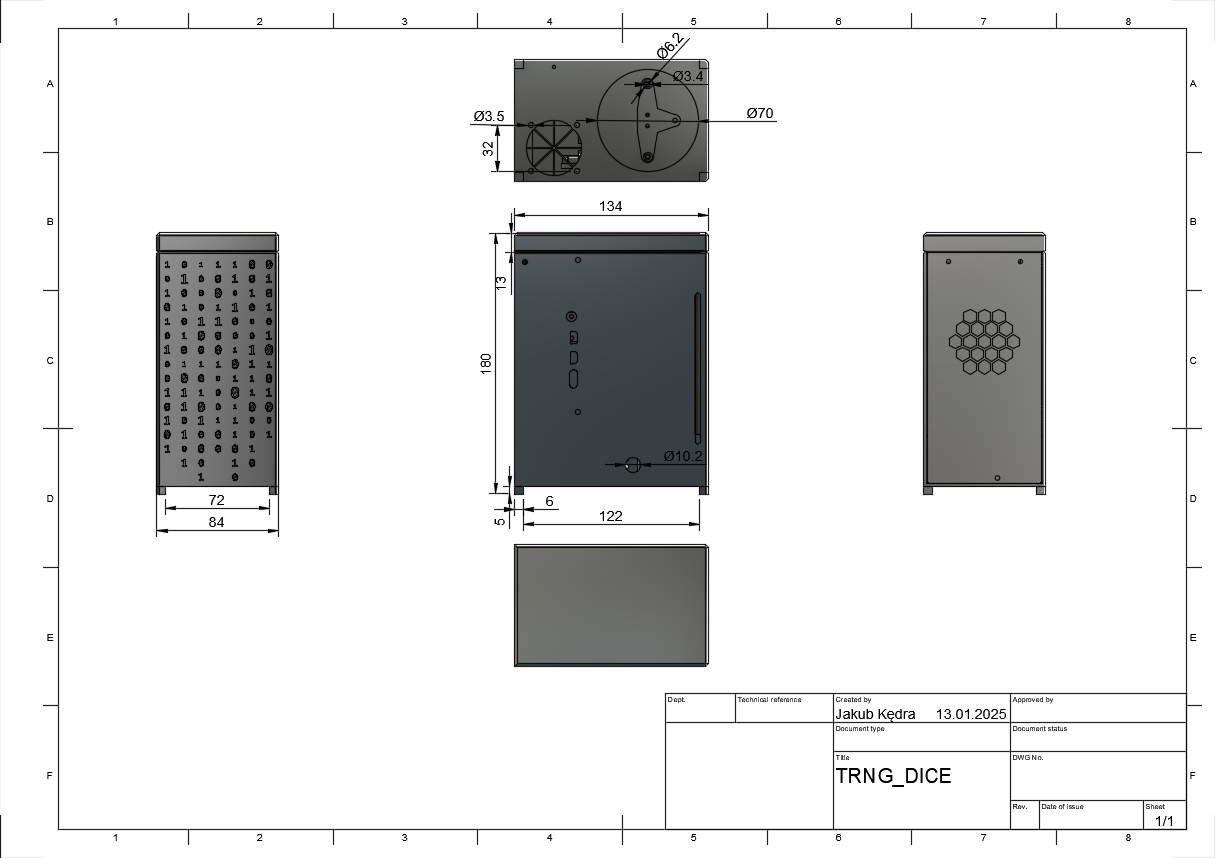
\includegraphics[width=0.95\linewidth]{chapters/03-praca-wlasna/figures/wymiary.png}
    \caption{\label{fig:wymiary}Wymiary zewnętrzne}
\end{figure}

\begin{figure}[H]
    \centering
    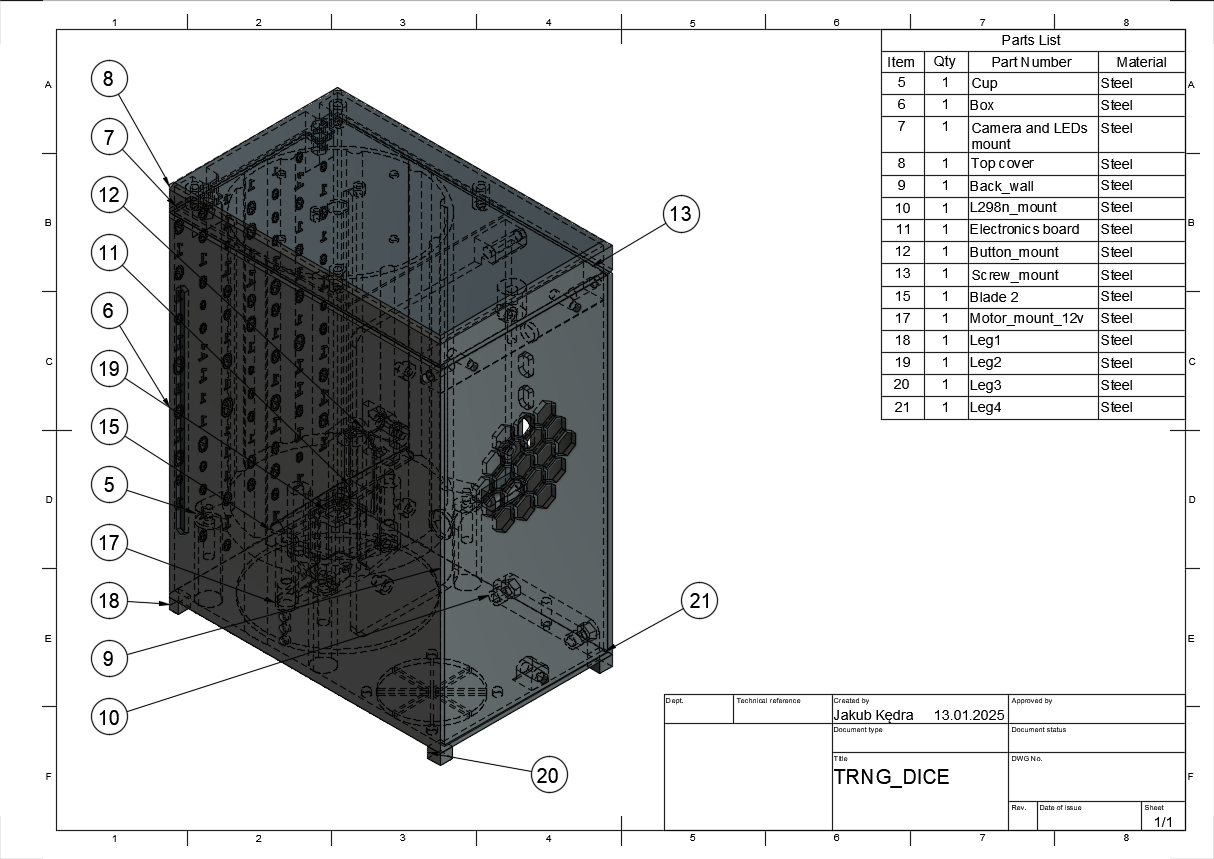
\includegraphics[width=0.95\linewidth]{chapters/03-praca-wlasna/figures/komponenty.png}
    \caption{\label{fig:komponenty}Komponenty robota}
\end{figure}

\subsection{Software}
bbbbbbbbbbbbbbbbbbbbb